\documentclass[12pt,a4paper]{article}

% --- Bezpatkový font (pdfLaTeX friendly) ---
\usepackage[T1]{fontenc}
\usepackage{nopageno}
\usepackage[utf8]{inputenc}

%img
\usepackage{graphicx}
\graphicspath{ {./img/} }


\IfFileExists{roboto.sty}{
	\usepackage[sfdefault]{roboto}
}{
	\IfFileExists{tgheros.sty}{\usepackage{tgheros}}{\usepackage[scaled=0.94]{helvet}}
}
\renewcommand{\familydefault}{\sfdefault}

% --- Jazyk, vzhled, barvy ---
\usepackage[czech]{babel}
\usepackage[a4paper,margin=2.5cm]{geometry}
\usepackage{microtype}
\usepackage{parskip}
\usepackage{xcolor}
\definecolor{main}{HTML}{004AAD}

% --- Odkazy ---
\usepackage{hyperref}
\hypersetup{colorlinks=true, linkcolor=main, urlcolor=main, citecolor=main}

% --- Grafika ---
\usepackage{graphicx}

% --- Nadpisy ---
\usepackage{titlesec}
\setlength{\parskip}{0.8em}
\setlength{\parindent}{0pt}

% Sekce a podsekce (bez "kapitol")
\titleformat{\section}
{\Large\bfseries\sffamily\color{main}}{\thesection}{0.8em}{}
\titleformat{\subsection}
{\large\bfseries\sffamily\color{main}}{\thesubsection}{0.6em}{}

% --- Obsah (tocloft) ---
\usepackage{tocloft}
\renewcommand{\cfttoctitlefont}{\Huge\bfseries\sffamily\color{main}}
\renewcommand{\cftsecfont}{\color{main}}
\renewcommand{\cftsecpagefont}{\color{main}}
\renewcommand{\cftsubsecfont}{\color{main}}
\renewcommand{\cftsubsecpagefont}{\color{main}}
\renewcommand{\cftdotsep}{1.2}
\renewcommand{\cftsecleader}{\color{main}\cftdotfill{\cftdotsep}}
\renewcommand{\cftsubsecleader}{\color{main}\cftdotfill{\cftdotsep}}

\titleformat{\subsubsection}[runin] % "runin" = inline nadpis (v textu), lze změnit na "hang"
{\sffamily\color{main}}             % styl – sans-serif, modrá
{}                                 % bez čísla
{0pt}                              % mezera mezi číslem (není) a textem
{}                                 % kód před textem

% --- Zápatí s číslem stránky ---
\usepackage{fancyhdr}
\pagestyle{fancy}
\fancyhf{}
\renewcommand{\headrulewidth}{0pt}
\fancyfoot[C]{\thepage}

% --- Meta pro titulní stranu ---
\newcommand{\docTitle}{Název dokumentace}
\newcommand{\docAuthor}{Tvoje společnost}
\newcommand{\docYear}{2025}

% --- Titulní strana ---
\newcommand{\makecleancover}{%
	\begin{titlepage}
		\thispagestyle{empty}
		\centering
		{\color{main}\rule{\textwidth}{2pt}\par}
		\vspace{2.6cm}
		{\fontsize{28pt}{32pt}\selectfont\bfseries\sffamily\color{main}\docTitle\par}
		\vspace{0.8cm}
		{\large\sffamily \docAuthor\par}
		\vspace{0.4cm}
		{\large\sffamily \docYear\par}
		\vfill
		\IfFileExists{logo.pdf}{
			\makebox[\textwidth]{
\includegraphics[width=0.25\textwidth]{logo.pdf}}
		}{
			\IfFileExists{logo.png}{\makebox[\textwidth]{
\includegraphics[width=0.25\textwidth]{logo.png}}{}}
		}
		{\color{main}\rule{\textwidth}{2pt}\par}
	\end{titlepage}
}

% ================== DOKUMENT ==================
\begin{document}
	
	\renewcommand{\docTitle}{Božské tóny v Krušnohoří}
	\renewcommand{\docAuthor}{ViasWebs}
	\renewcommand{\docYear}{2025}
	
	\makecleancover
	
	% Obsah
	\thispagestyle{empty}
	\tableofcontents
	\clearpage
	
	% Číslování od první sekce (pokud chceš čísla; máš ale \usepackage{nopageno} – ten je vypíná globálně)
	\setcounter{page}{1}
	
	\section{Funkční přehled webu}
	
	\subsection{O projektu}
	Záložka \emph{O projektu} na webu poskytuje uživatelům rychlý vhled do účelu a rozsahu iniciativy. Typicky zde najdou:
	
	\begin{itemize}
		\item \textbf{Stručné představení} — co je projekt \emph{Božské tóny v Krušnohoří} a proč vznikl.
		\item \textbf{Cíle a směřování} — hlavní motivace, zaměření a zapojení regionu.
		\item \textbf{Klíčové aktivity} — výzkumná studie, výstava, kalendář akcí, materiály ke stažení.
		\item \textbf{Pro koho projekt je} — cílové skupiny, zapojení komunit, regionální partnerství.
		\item \textbf{Partnery} — odkazy na jednotlivá místa a zapojené partnery projektu.
	\end{itemize}
	
	\subsection{Aktuality}
	Sekce \emph{Aktuality} zobrazuje chronologicky řazené příspěvky s náhledem
	(titulek, datum, autor) a odkazem na detail. Na úvodní stránce se vybrané
	novinky zobrazují formou karet (\uv{Příspěvky z akcí}).
	
	\subsection{Kalendář akcí}
	Kalendář podporuje zobrazení \textbf{Měsíc/Týden/Den}, navigaci mezi obdobími
	(\uv{Předchozí}, \uv{Dnes}) a filtr kategorií. Nechybí \textbf{Zobrazení pro tisk}
	pro snadnou distribuci programu. V přehledu se zobrazují aktuální měsíce
	a plánované události.
	
	\subsection{Ke stažení}
	Sekce \emph{Ke stažení} slouží pro publikaci dokumentů a materiálů (např. tiskové
	sestavy, podklady pro partnery). Stránka je přístupná z horní navigace a obsah
	je členěn pro snadné stažení.
	
	\subsection{Kontakty a partneři}
	Záložka \emph{Kontakty} poskytuje kontaktní informace; na úvodu je blok
	\emph{Partneři} s logy a odkazy. V patičce je uveden provozovatel a autor designu.
	
	\subsection{Jazyky a sdílení}
	Přepínač \textbf{CS/DE} umožňuje rychlé přepnutí obsahu mezi češtinou a němčinou.
	Na úvodní stránce je také odkaz na \emph{Facebook} pro sdílení a sledování novinek.
	
	\subsection{Cookies a tisk}
	Web zobrazuje informační lištu o cookies s volbou souhlasu.
	U kalendáře je k dispozici speciální \emph{tiskové zobrazení} pro pohodlný export programu.
	
	\newpage
	\section{Technické řešení webu}
	Web je postaven na redakčním systému \textbf{WordPress}, který umožňuje snadnou
	správu obsahu a dlouhodobou udržitelnost. Pro tvorbu vzhledu je využit
	šablonovací systém \textbf{Elementor}, jenž poskytuje vizuální rozhraní pro editaci
	a rychlé sestavování sekcí bez zásahů do kódu. Web je plně \textbf{responzivní}
	(PC, tablet, mobil) a \textbf{lokalizovaný} pro češtinu a němčinu
	(přeshraniční charakter projektu) pomocí externí domény \url{http://www.goettlicheklaenge.de/}.
	\subsection*{Hosting}
	Provoz webu je zajištěn přes hostingovou společnost \textbf{Blueboard}.
	Správu hostingu i souvisejících služeb zajišťuje přímo zákazník.
	
	\newpage
	\section{Wordpress}
	Tento manuál slouží pro základní správu webu postaveného na systému WordPress.
	
	\subsection{Správa účtů a oprávnění}
	WordPress umožňuje více uživatelů s různými oprávněními.
	\begin{enumerate}
		\item \textbf{Přihlášení:} Přes adresu \url{https://bozsketony.cz/wp-admin}
		\item \textbf{Pro zobrazení} uživatelů klikněte v levém menu na položku „Uživatelé“.
	\end{enumerate}

	\begin{figure}[htp]
		\centering
		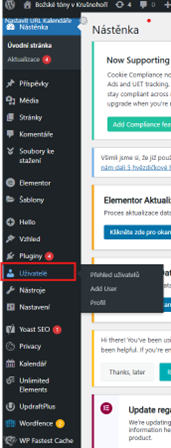
\includegraphics[width=6cm]{role}
		\caption{Ukázka správy rolí ve WordPressu}
		\label{fig:role}
	\end{figure}
	
	\newpage
	Zde můžete upravit, případně vytvořit nové uživatele. Pro přidání uživatele klikněte na „Add User“ a vyplňte požadované údaje ve formuláři.
	
	\subsection{Systémové role}
	Redakční systém WordPress využívá předem definované role. Níže je popis jednotlivých rolí:
	
	\subsubsection*{Administrátor}
	\begin{enumerate}
		\item \textbf{Popis:} Má neomezená práva k celému webu.
		\item \textbf{Práva:} Může instalovat a mazat pluginy a šablony, spravovat uživatele, upravovat nastavení webu a publikovat, editovat či mazat jakýkoliv obsah.
		\item \textbf{Kdy použít:} Role pro majitele webu nebo hlavního správce. Je vhodné mít jen jednoho, maximálně dva administrátory.
	\end{enumerate}
	
	\subsubsection*{Šéfredaktor}
	\begin{enumerate}
		\item \textbf{Popis:} Má plnou kontrolu nad obsahem.
		\item \textbf{Práva:} Může publikovat, upravovat a mazat jakékoliv příspěvky (včetně příspěvků jiných autorů), spravovat rubriky a štítky a moderovat komentáře. Nemůže ale spravovat pluginy, šablony nebo uživatele.
		\item \textbf{Kdy použít:} Ideální pro hlavního editora nebo manažera obsahu, který má na starosti celý publikační plán.
	\end{enumerate}
	
	\subsubsection*{Redaktor}
	\begin{enumerate}
		\item \textbf{Popis:} Může spravovat a publikovat své vlastní příspěvky.
		\item \textbf{Práva:} Může psát, publikovat, upravovat a mazat pouze své vlastní příspěvky. Může také nahrávat soubory (obrázky, dokumenty) a moderovat komentáře ke svým příspěvkům.
		\item \textbf{Kdy použít:} Vhodné pro autory, kteří píší pravidelně a mají právo publikovat svůj obsah bez schválení.
	\end{enumerate}\subsection*{Systémové role}
	Redakční systém WordPress využívá předem definované role. Níže je popis jednotlivých rolí:
	
	\newpage
	\subsubsection*{Administrátor}
	\begin{enumerate}
	\item \textbf{Popis:} Má neomezená práva k celému webu.
	\item \textbf{Práva:} Může instalovat a mazat pluginy a šablony, spravovat uživatele, upravovat nastavení webu a publikovat, editovat či mazat jakýkoliv obsah.
	\item \textbf{Kdy použít:} Role pro majitele webu nebo hlavního správce. Je vhodné mít jen jednoho, maximálně dva administrátory.
	\end{enumerate}
	
	\subsubsection*{Šéfredaktor}
	\begin{enumerate}
	\item \textbf{Popis:} Má plnou kontrolu nad obsahem.
	\item \textbf{Práva:} Může publikovat, upravovat a mazat jakékoliv příspěvky (včetně příspěvků jiných autorů), spravovat rubriky a štítky a moderovat komentáře. Nemůže ale spravovat pluginy, šablony nebo uživatele.
	\item \textbf{Kdy použít:} Ideální pro hlavního editora nebo manažera obsahu, který má na starosti celý publikační plán.
	\end{enumerate}
	
	\subsubsection*{Redaktor}
	\begin{enumerate}
	\item \textbf{Popis:} Může spravovat a publikovat své vlastní příspěvky.
	\item \textbf{Práva:} Může psát, publikovat, upravovat a mazat pouze své vlastní příspěvky. Může také nahrávat soubory (obrázky, dokumenty) a moderovat komentáře ke svým příspěvkům.
	\item \textbf{Kdy použít:} Vhodné pro autory, kteří píší pravidelně a mají právo publikovat svůj obsah bez schválení.
	\end{enumerate}
	
	\subsubsection*{Spolupracovník}
	\begin{enumerate}
	\item \textbf{Popis:} Může psát, ale nemůže publikovat.
	\item \textbf{Práva:} Může psát a upravovat své vlastní příspěvky, ale k jejich publikování je nutné schválení redaktorem nebo administrátorem. Nemůže nahrávat soubory ani spravovat komentáře.
	\item \textbf{Kdy použít:} Skvělé pro externí autory nebo hosty, jejichž příspěvky je potřeba zkontrolovat a schválit před zveřejněním.
	\end{enumerate}
	
	\subsubsection*{Návštěvník}
	\begin{enumerate}
	\item \textbf{Popis:} Standardní role pro nepřihlášeného uživatele, nebo speciálně nastavená role s velmi omezenými právy.
	\item \textbf{Práva:} Obvykle nemá žádná práva k úpravám obsahu. Může pouze číst a komentovat (pokud je to povoleno).
	\item \textbf{Kdy použít:} Role pro každého, kdo navštíví web bez přihlášení. V některých případech se používá i pro přihlášené uživatele, kteří mají právo jen číst exkluzivní obsah.
	\end{enumerate}
	
	\subsection*{Speciální role pro SEO (plugin Yoast SEO)}
	
	\subsubsection*{SEO Manager}
	\begin{enumerate}
	\item \textbf{Popis:} Má plný přístup ke všem funkcím a nastavením pluginu Yoast SEO.
	\item \textbf{Práva a možnosti:}  
	- Úprava globálních nastavení (titulky, meta popisky, RSS, sociální sítě).  
	- Přístup k nástrojům Yoast SEO (editor souborů, přesměrování, import/export).  
	- Ovládání nastavení indexování a crawlingu (noindex, nofollow).  
	- Možnost editovat SEO analýzy všech příspěvků a stránek.  
	- Přístup k pokročilým nastavením (schema markup, integrace s nástroji).
	\item \textbf{Kdy použít:} Ideální pro SEO specialistu, marketingového manažera nebo webmastera.
	\end{enumerate}
	
	\subsubsection*{SEO Editor}
	\begin{enumerate}
	\item \textbf{Popis:} Má omezený přístup, zaměřuje se na optimalizaci obsahu.
	\item \textbf{Práva a možnosti:}  
	- Úprava SEO analýzy a čitelnosti pro vlastní příspěvky.  
	- Nastavení klíčových frází, meta popisků a SEO titulků.  
	- Nemá přístup k globálním ani pokročilým nastavením.
	\item \textbf{Kdy použít:} Vhodné pro autory, redaktory nebo copywritery, kteří optimalizují obsah pro vyhledávače.
	\end{enumerate}
	
	
	\subsubsection*{Spolupracovník}
	\begin{enumerate}
		\item \textbf{Popis:} Může psát, ale nemůže publikovat.
		\item \textbf{Práva:} Může psát a upravovat své vlastní příspěvky, ale k jejich publikování je nutné schválení redaktorem nebo administrátorem. Nemůže nahrávat soubory ani spravovat komentáře.
		\item \textbf{Kdy použít:} Skvělé pro externí autory nebo hosty, jejichž příspěvky je potřeba zkontrolovat a schválit před zveřejněním.
	\end{enumerate}
	
	\subsubsection*{Návštěvník}
	\begin{enumerate}
		\item \textbf{Popis:} Standardní role pro nepřihlášeného uživatele, nebo speciálně nastavená role s velmi omezenými právy.
		\item \textbf{Práva:} Obvykle nemá žádná práva k úpravám obsahu. Může pouze číst a komentovat (pokud je to povoleno).
		\item \textbf{Kdy použít:} Role pro každého, kdo navštíví web bez přihlášení. V některých případech se používá i pro přihlášené uživatele, kteří mají právo jen číst exkluzivní obsah.
	\end{enumerate}
	
	\subsection*{Speciální role pro SEO (plugin Yoast SEO)}
	
	\subsubsection*{SEO Manager}
	\begin{enumerate}
		\item \textbf{Popis:} Má plný přístup ke všem funkcím a nastavením pluginu Yoast SEO.
		\item \textbf{Práva a možnosti:}  
		- Úprava globálních nastavení (titulky, meta popisky, RSS, sociální sítě).  
		- Přístup k nástrojům Yoast SEO (editor souborů, přesměrování, import/export).  
		- Ovládání nastavení indexování a crawlingu (noindex, nofollow).  
		- Možnost editovat SEO analýzy všech příspěvků a stránek.  
		- Přístup k pokročilým nastavením (schema markup, integrace s nástroji).
		\item \textbf{Kdy použít:} Ideální pro SEO specialistu, marketingového manažera nebo webmastera.
	\end{enumerate}
	
	\subsubsection*{SEO Editor}
	\begin{enumerate}
		\item \textbf{Popis:} Má omezený přístup, zaměřuje se na optimalizaci obsahu.
		\item \textbf{Práva a možnosti:}  
		- Úprava SEO analýzy a čitelnosti pro vlastní příspěvky.  
		- Nastavení klíčových frází, meta popisků a SEO titulků.  
		- Nemá přístup k globálním ani pokročilým nastavením.
		\item \textbf{Kdy použít:} Vhodné pro autory, redaktory nebo copywritery, kteří optimalizují obsah pro vyhledávače.
	\end{enumerate}
	
	\subsection{Aktualizace WordPressu a pluginů}
	Pravidelné aktualizace všech dostupných prvků jsou důležité pro bezpečnost a funkčnost webu. Aktualizace doporučujeme provádět pravidelně \textbf{alespoň 1x za měsíc}.
	
	\begin{figure}[htp]
		\centering
		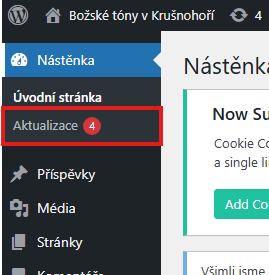
\includegraphics[width=5cm]{WPupdate1}
		\caption{Aktualizace ve WordPressu - lišta}
		\label{fig:role}
	\end{figure}
	
	Klikněte na Aktualizovat nyní, pokud je dostupná nová verze. Následně klikněte na Aktualizovat nyní, pokud je dostupná nová verze.
	
	\begin{figure}[htp]
		\centering
		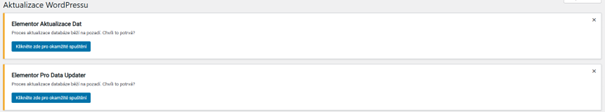
\includegraphics[width=18cm]{WPupdatesite}
		\caption{Aktualizace ve WordPressu - notifikace aktualizací}
		\label{fig:role}
	\end{figure}
	
	\subsection{Aktualizace pluginů}
	Aktualizace pluginů probíhá automaticky, nicméně v případě, že by automatická aktualizace selhala, může být nutné aktualizaci spustit ručně. Pro ruční spuštění aktualizace pluginů jděte níže na stránce „Aktualizace“ viz. Aktualizace WordPressu. Vyberte pluginy, které chcete aktualizovat a klikněte na „Aktualizovat pluginy“.
	
		
	\begin{figure}[htp]
		\centering
		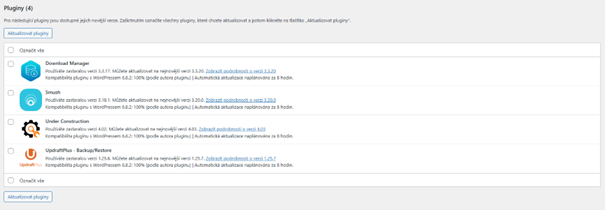
\includegraphics[width=18cm]{WPupdateplugin}
		\caption{Aktualizace ve WordPressu - pluginy}
		\label{fig:role}
	\end{figure}
	
	\textbf{Doporučení:} Před větší aktualizací (např. WordPressu) udělejte zálohu pomocí pluginu \textbf{UpdraftPlus}.
	
	\subsection{Zálohování}
	Pro vytvoření zálohy stačí v levé sekci zvolit položku „UpdraftPlus“. Jedná se o doplněk, který vytvoří zálohu webu, kterou je později na vyžádání schopen obnovit. Záloha je vytvořena a odeslána na FTP server \url{viaswebs.cz}, hostovaný společností BlueBoard.
	
	\newpage
	\begin{figure}[htp]
		\centering
		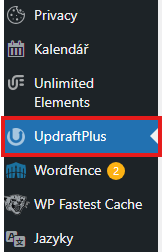
\includegraphics[width=5cm]{WPbackupmenu}
		\caption{Aktualizace ve WordPressu - zálohování}
		\label{fig:role}
	\end{figure}
	
	Zde pouze kliknete na „Zálohovat nyní“ a tím spustíte proces zálohování.
	
	\begin{figure}[htp]
		\centering
		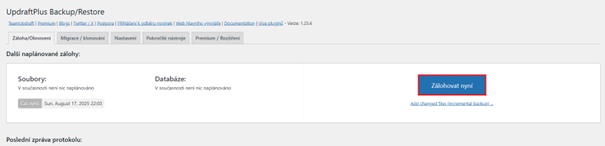
\includegraphics[width=17cm]{WPmakebackup}
		\caption{Aktualizace ve WordPressu - vytvoření zálohy}
		\label{fig:role}
	\end{figure}
	
	Pro obnovení webu do stavu před aktualizací, nebo jakoukoli nechtěnou změnou stačí vybrat v seznamu zálohu, kterou chcete obnovit a kliknout na „Obnovit“ ve sloupci „Akce“.
	
	\begin{figure}[htp]
		\centering
		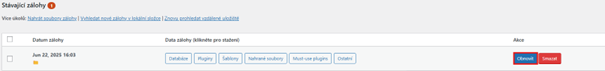
\includegraphics[width=17cm]{WPrestore}
		\caption{Aktualizace ve WordPressu - obnova zálohy}
		\label{fig:role}
	\end{figure}
	
	\newpage
	\subsection{Použité pluginy}
	Pokud budete chtít nainstalovat nový plugin, nebo deaktivovat / nastavit stávající, v záložce menu vyberte položku “Pluginy”.
			
	\begin{figure}[htp]
		\centering
		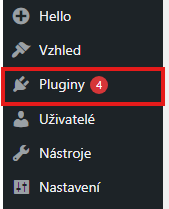
\includegraphics[width=5cm]{WPplugins}
		\caption{Pluginy ve Wordpressu - výčet}
		\label{fig:role}
	\end{figure}
	

	Web využívá následující pluginy:
	\begin{enumerate}
		\item \textbf{Autoptimize} – zrychlení webu (optimalizace kódu)
		\item \textbf{Better Search Replace} – hromadná úprava textů/dat v databázi (používat jen administrátor)
		\item \textbf{Category Posts in Custom Menu} – zobrazení kategorií v menu
		\item \textbf{Clear Autoptimize Cache Automatically} – automatické mazání cache Autoptimize
		\item \textbf{Connect Polylang for Elementor} – propojení jazyků (Polylang) s Elementorem
		\item \textbf{Cookie Notice \& Compliance for GDPR / CCPA} – lišta se souhlasem s cookies
		\item \textbf{Download Manager} – správa a stahování souborů
		\item \textbf{Elementor + Elementor Pro} – vizuální editor stránek
		\item \textbf{HTTP Headers} – bezpečnostní hlavičky
		\item \textbf{Klasický editor} – původní editor místo Gutenberg bloků
		\item \textbf{My Calendar} – správa událostí a kalendáře
		\item \textbf{Pages with category and tag} – možnost přiřadit stránkám štítky a kategorie
		\item \textbf{Polylang} – vícejazyčnost webu
		\item \textbf{Smush} – optimalizace obrázků
		\item \textbf{Under Construction} – režim „stránka v přípravě“
		\item \textbf{Unlimited Elements for Elementor} – další widgety do Elementoru
		\item \textbf{UpdraftPlus} – zálohování a obnova webu
		\item \textbf{Wordfence Security} – ochrana proti útokům
		\item \textbf{WP Fastest Cache} – zrychlení webu (cachování)
		\item \textbf{Yoast SEO} – nastavení pro vyhledávače (SEO)
	\end{enumerate}
	
	Mezi pluginy (kormě šablonovacího nástroje Elementor Pro) se nenachází žádný placený/licencovaný plugin, který by vyžadoval další správu.
	
	\subsection{Vymazání cache}
	Někdy se stane, že se na webu provede změna (např. úprava textu, obrázku, menu nebo designu), ale návštěvníci pořád vidí starou verzi stránky. To je způsobeno tím, že se jim zobrazuje uložená verze v cache. Cache je paměťová schránka, do které si web ukládá části stránek, aby se načítaly rychleji. Díky tomu se web návštěvníkům zobrazí během okamžiku, aniž by se musel pokaždé celý znovu načítat.
	
	Vymazání cache znamená, že dojde ke smazání uložených starých verzí stránek, tím se vynutí, aby se načetla aktuální verze webu.
	
	\textit{Kdy vymazat cache?}
	\begin{enumerate}
	\item Po úpravě obsahu (texty, obrázky, odkazy), pokud změny nejsou vidět.
	
	\item Po úpravě designu v Elementoru nebo šabloně.
	Po aktualizaci pluginů či WordPressu, aby se načetly nové verze souborů.
	
	\item Když se web chová „divně“ – načítají se rozbité styly, staré obrázky nebo prázdné bloky.

	\end{enumerate}
	
	\textit{Jak vymazat cache?}
	
	Menu: WP Fastest Cache → Smazat cache a minifikovat CSS/JS
	
	
	\newpage
	\section{Redakční IS}
	
	
	
	
	
	
	
	
	
	
	
	
\end{document}
